% =====================================================================
%  AI6127 Group Assignment — Group 20
%  Conversational RAG Product Recommender (two-column paper format)
%  Compiles with pdfLaTeX (Overleaf default) or XeLaTeX; run twice.
%  Fill in the [placeholders] in the title block below.
% =====================================================================
\documentclass[10pt,a4paper,twocolumn]{article}

\usepackage[a4paper,top=2cm,bottom=2.2cm,left=1.7cm,right=1.7cm,columnsep=0.6cm]{geometry}
\usepackage{iftex}
\ifPDFTeX
  % ---- pdfLaTeX (Overleaf default) ----
  \usepackage[utf8]{inputenc}
  \usepackage[T1]{fontenc}
  \IfFileExists{newtxtext.sty}{\usepackage{newtxtext}}{\usepackage{times}}
  % Chinese snippets in examples (\zh{...})
  \IfFileExists{CJKutf8.sty}{\usepackage{CJKutf8}\def\haveCJK{}}{}
  \ifdefined\haveCJK
    \newcommand{\zh}[1]{\begin{CJK}{UTF8}{gbsn}#1\end{CJK}}
  \else
    \newcommand{\zh}[1]{[Chinese text]}
  \fi
\else
  % ---- XeLaTeX / LuaLaTeX ----
  \usepackage{fontspec}
  \IfFontExistsTF{TeX Gyre Termes}{\setmainfont{TeX Gyre Termes}}{}
  \IfFontExistsTF{TeX Gyre Heros}{\setsansfont{TeX Gyre Heros}}{}
  \IfFontExistsTF{Noto Serif CJK SC}
    {\newfontfamily\zhfont{Noto Serif CJK SC}}
    {\newfontfamily\zhfont{FandolSong-Regular.otf}}
  \newcommand{\zh}[1]{{\zhfont #1}}
\fi
\usepackage{newunicodechar}
\newunicodechar{κ}{\ensuremath{\kappa}}
\newunicodechar{→}{\ensuremath{\rightarrow}}
\newunicodechar{≤}{\ensuremath{\leq}}
\newunicodechar{≥}{\ensuremath{\geq}}
\newunicodechar{−}{\ensuremath{-}}
\newunicodechar{×}{\ensuremath{\times}}

\usepackage{amsmath,amssymb}
\usepackage{graphicx}
\usepackage{booktabs,tabularx,makecell,multirow}
\usepackage[font=small,labelfont=bf,skip=4pt]{caption}
\usepackage{enumitem}
\setlist{nosep,leftmargin=*}
\usepackage{titlesec}
\titleformat{\section}{\large\bfseries}{\thesection}{0.6em}{}
\titleformat{\subsection}{\normalsize\bfseries}{\thesubsection}{0.5em}{}
\titlespacing*{\section}{0pt}{9pt plus 2pt}{4pt}
\titlespacing*{\subsection}{0pt}{6pt plus 2pt}{3pt}
\usepackage{microtype}
\usepackage[hidelinks]{hyperref}
\usepackage{xurl}
\usepackage{xcolor}
\newcommand{\code}[1]{\texttt{\small #1}}
\setlength{\tabcolsep}{4pt}
\renewcommand{\arraystretch}{1.08}
\setlength{\textfloatsep}{8pt plus 2pt}
\setlength{\floatsep}{6pt plus 2pt}
\setlength{\dbltextfloatsep}{8pt plus 2pt}
% float placement: allow large floats at the top of pages
\renewcommand{\topfraction}{0.9}\renewcommand{\bottomfraction}{0.6}
\renewcommand{\dbltopfraction}{0.92}\renewcommand{\textfraction}{0.05}
\renewcommand{\floatpagefraction}{0.75}\renewcommand{\dblfloatpagefraction}{0.75}
\setcounter{topnumber}{3}\setcounter{dbltopnumber}{2}\setcounter{totalnumber}{5}

\begin{document}

% ============================ TITLE PAGE ==============================
\begin{titlepage}
\centering
\vspace*{0.8cm}
{\large AI6127 Deep Neural Networks for Natural Language Processing\par}
\vspace{4pt}
{\large Group Assignment 2026\par}
\vspace{1.6cm}
{\fontsize{24}{30}\selectfont\bfseries A Conversational RAG Product Recommender\\[4pt] that Asks Before It Recommends\par}
\vspace{1.3cm}
{\LARGE\bfseries Group 20\par}
\vspace{1.0cm}

{\large
\renewcommand{\arraystretch}{1.55}
\begin{tabular}{@{}c p{7.2cm} p{4.2cm}@{}}
\toprule
 & \textbf{Name} & \textbf{Matriculation No.}\\
\midrule
1 & {[Member 1 name]} & {[U0000000A]}\\
2 & {[Member 2 name]} & {[U0000000A]}\\
3 & {[Member 3 name]} & {[U0000000A]}\\
4 & {[Member 4 name]} & {[U0000000A]}\\
5 & {[Member 5 name]} & {[U0000000A]}\\
\bottomrule
\end{tabular}\par}
\vspace{1.2cm}

{\renewcommand{\arraystretch}{1.5}
\begin{tabular}{@{}>{\raggedright\arraybackslash}p{5.6cm} >{\raggedright\arraybackslash}p{9.4cm}@{}}
\textbf{Data} (knowledge base, queries, retrieved results, evaluation dataset, generated answers): & \textit{[link to the data zip — replace with} \texttt{\textbackslash url\{...\}}\textit{]}\\
\textbf{Code} (source code, libraries, README): & \textit{[link to the code zip — replace with} \texttt{\textbackslash url\{...\}}\textit{]}\\
\textbf{Repository:} & \url{https://github.com/lsy640/AI6127-RAG}\\
\end{tabular}\par}
\vspace{1.2cm}

\begin{minipage}{0.86\textwidth}
\small\textbf{Abstract.} Shoppers rarely state a complete need in their first message. We build a retrieval-augmented assistant over 15,000 Amazon products that decides at every turn whether to ask a clarifying question or to recommend, and grounds every recommendation in retrieved evidence. Retrieval combines BM25 and bge-m3 dense search over field-level chunks with reciprocal rank fusion, metadata and date filters and a cross-encoder re-ranker (human-judged P@5 0.62 → 0.90). The downstream agent adds clarification, conversational query rewriting with constraint-to-filter mapping, and an evidence check with claim-level self-verification. On 169 unique simulated dialogues it reaches 0.876 success within five turns versus 0.586 without clarification, with LLM-judged faithfulness of 0.998. The evaluation set has 1,313 unique human-labelled records (three annotators, 95.8\,\% agreement).
\end{minipage}
\vfill
\end{titlepage}

% =====================================================================
\section{System Overview}
A single message such as \emph{``I need some shoes''} says nothing about the type, the wearer or the budget. Our agent therefore runs the pipeline of Fig.~\ref{fig:arch} at every turn: (1)~an LLM tracks the need as slots \{\code{product\_type}, \code{audience}, \code{age}, \code{price\_max}, \code{material}\} and rewrites the dialogue into a standalone English query; (2)~hard constraints become metadata filters; (3)~hybrid retrieval and re-ranking produce candidates; (4)~the agent decides to \emph{ask}, \emph{recommend} or report that \emph{nothing matches}; (5)~before recommending it checks the evidence, generates a JSON answer with product and evidence IDs, and verifies each claim. The LLM is DeepSeek \code{deepseek-flash} with reasoning disabled (temperature 0).

\begin{figure*}[t]
\centering
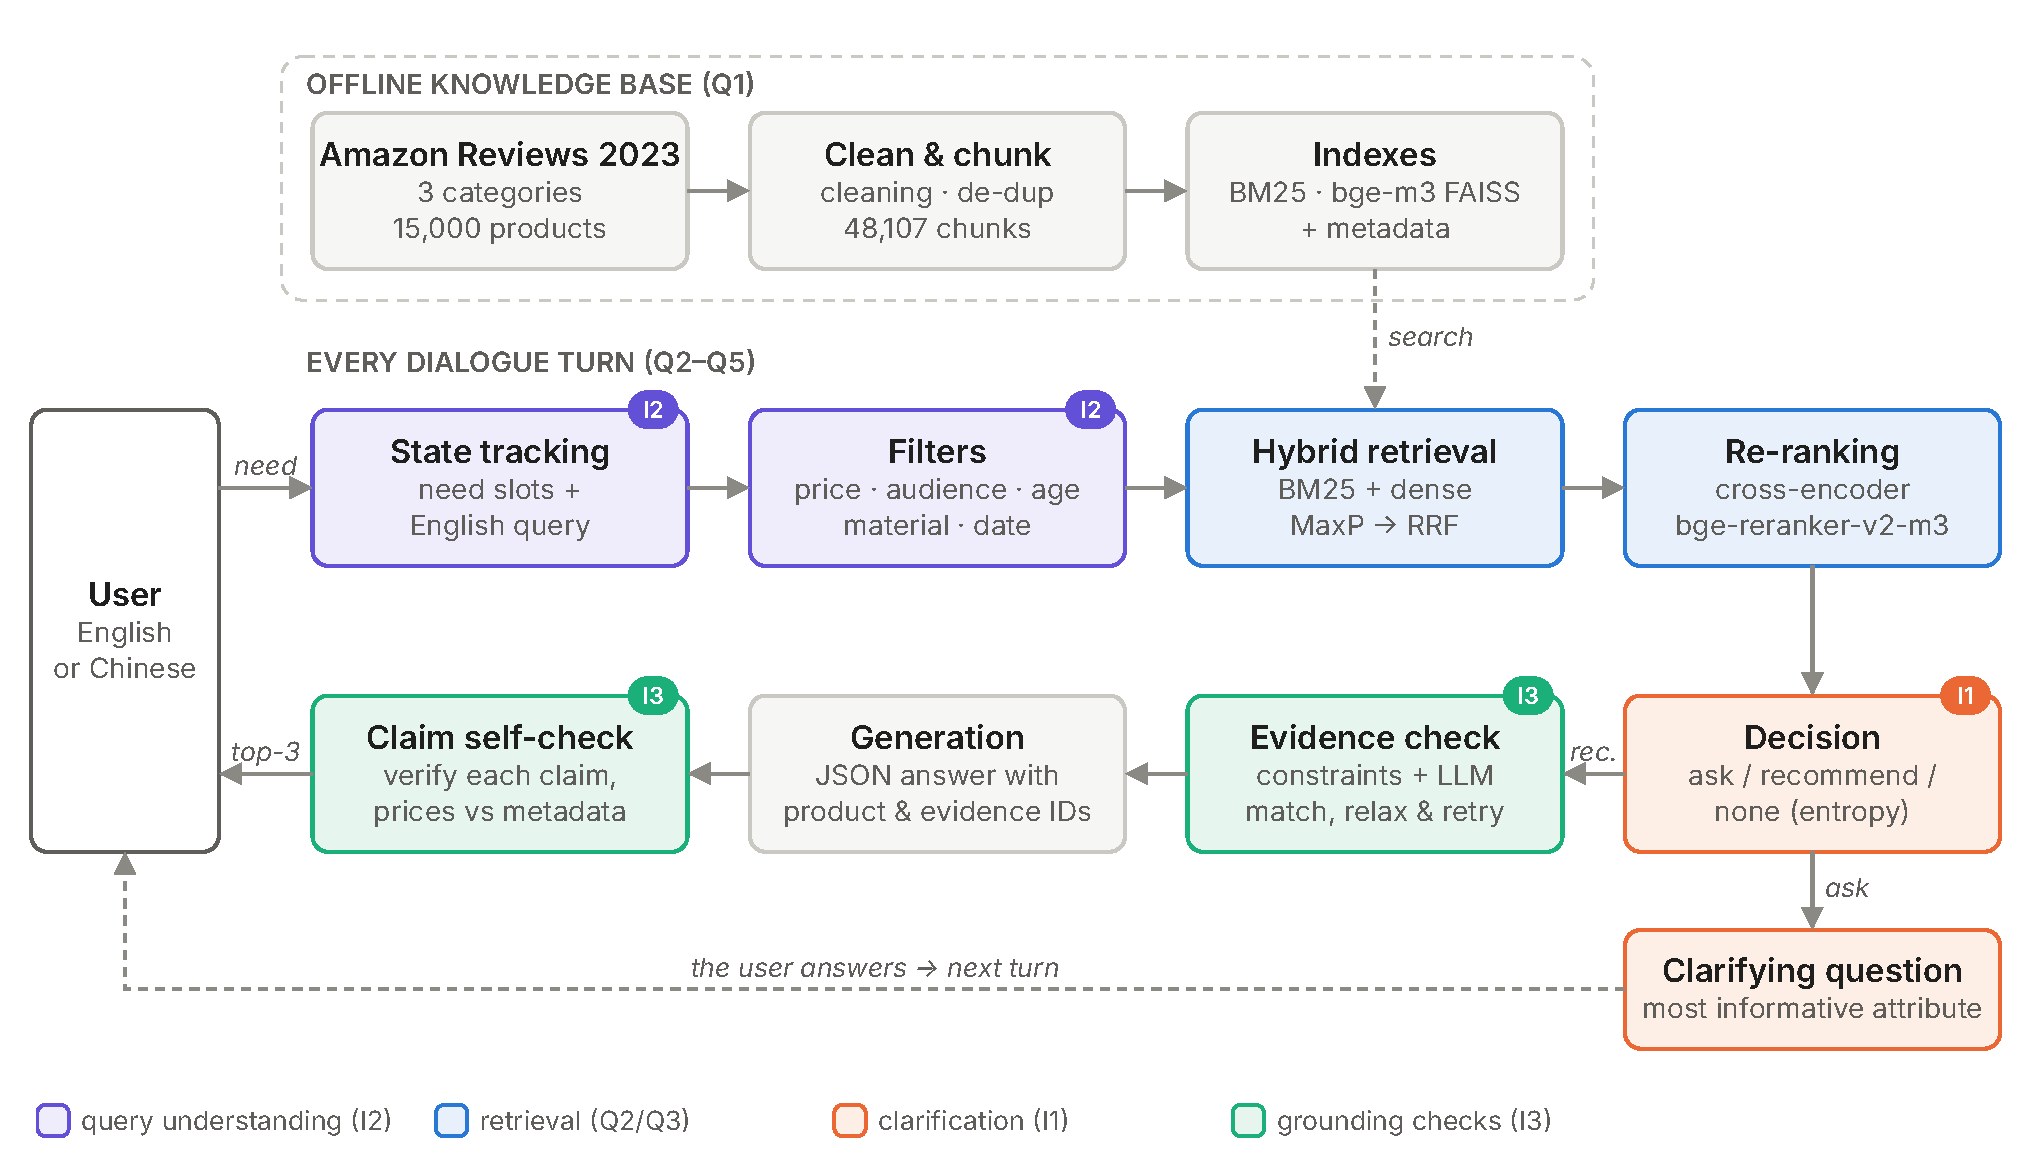
\includegraphics[width=\textwidth]{figures/fig_architecture.pdf}
\caption{System architecture. Top: offline knowledge base (Q1). Middle and bottom: the pipeline executed at every dialogue turn; colours mark query understanding (I2), retrieval (Q2/Q3), clarification (I1) and grounding checks (I3).}
\label{fig:arch}
\end{figure*}

% =====================================================================
\section{Knowledge Base (Q1)}
\textbf{Gathering.} We use the McAuley Lab \emph{Amazon Reviews 2023} product metadata~\cite{hou2024} for Clothing, Shoes \& Jewelry (7.2\,M products), Home \& Kitchen (3.7\,M) and Toys \& Games (0.9\,M), streamed from the public \code{.jsonl.gz} dumps. A product is valid if title, features, description, categories, details, price, rating, rating count and store are all non-empty (11.6\,\%, 20.1\,\% and 30.2\,\% of the three files). We draw 5,000 products per category by \emph{reservoir sampling over the whole file}; taking the first valid products would be biased (the first 30k Clothing items are 25\,\% valid versus 11.6\,\% overall).

\textbf{Cleaning and storage.} We strip HTML and decorative symbols, drop noisy specification keys (e.g.\ Best Sellers Rank, model numbers), and de-duplicate by \code{parent\_asin} and normalised title. Semantic fields (title, categories, features, description, specifications) form the indexed text; price, rating, review count, store, category path, release date and attributes are kept as structured metadata for filtering and evidence headers, so that numbers do not dilute embeddings.

\textbf{Chunking.} Each product is split into title-prefixed \emph{field-level} chunks: \emph{overview} (categories and features), \emph{description} (200-word windows, 40-word overlap) and \emph{specs}. Retrieval scores chunks and merges them to products (MaxP); the generator receives the product text with a price/rating header.

\textbf{Application.} Users chat in English or Chinese; the system asks follow-up questions and recommends products with grounded reasons (Fig.~\ref{fig:ui}). Table~\ref{tab:corpus} gives the corpus statistics.

\begin{table}[!htb]
\centering\small
\caption{Corpus statistics.}
\label{tab:corpus}
\begin{tabular}{@{}l r@{}}
\toprule
Documents (products) & 15,000\\
Chunks & 48,107\\
\quad overview/description/specs & 16,483/16,609/15,015\\
Words (whitespace tokens) & 3,589,422\\
Types (lower-cased alphanumeric) & 60,141\\
Words/product (mean/median/max) & 239 / 203 / 2,040\\
\bottomrule
\end{tabular}
\end{table}

% =====================================================================
\section{Retrieval System (Q2)}
\textbf{Sparse.} Okapi BM25 ($k_1{=}1.5$, $b{=}0.75$) stored as a pre-weighted SciPy sparse matrix with a normalising tokenizer (lower-casing, punctuation, stop-words); 0.2\,ms per query versus $\sim$100\,ms for \code{rank\_bm25}. \textbf{Dense.} \code{BAAI/bge-m3} (1024-d, multilingual) in a FAISS \code{IndexFlatIP}, encoded in fp16 on Apple Silicon (cosine to fp32 $\geq$ 0.9998). \textbf{Fusion.} Both rankings are merged to products and combined with reciprocal rank fusion (RRF, $k{=}60$)~\cite{cormack2009}.

\textbf{Interface.} A Gradio chat (Fig.~\ref{fig:ui}) shows the dialogue, the tracked need, the cited evidence and per-stage latency; a drop-down switches between the ablation configurations of Section~\ref{sec:q5}.

\textbf{Query speed.} Table~\ref{tab:speed} lists five queries (Apple M5, warm, median of 10 runs). Query encoding dominates; with cross-encoder re-ranking of the top-20 products the mean latency rises to 0.69\,s.

\begin{table}[!htb]
\centering\small
\caption{Latency of five queries (ms).}
\label{tab:speed}
\footnotesize
\begin{tabularx}{\columnwidth}{@{}X rrrr@{}}
\toprule
Query & BM25 & Encode & FAISS & Total\\
\midrule
waterproof men's hiking boots & 0.3 & 16.7 & 1.6 & 18.6\\
non-stick frying pan for induction stove & 0.2 & 16.7 & 1.6 & 18.5\\
board game for family night with kids & 0.2 & 16.5 & 1.6 & 18.4\\
sterling silver earrings for sensitive ears & 0.2 & 16.5 & 1.6 & 18.4\\
soft queen size bed sheets & 0.2 & 16.4 & 1.6 & 18.2\\
\bottomrule
\end{tabularx}
\end{table}

\begin{figure*}[t]
\centering
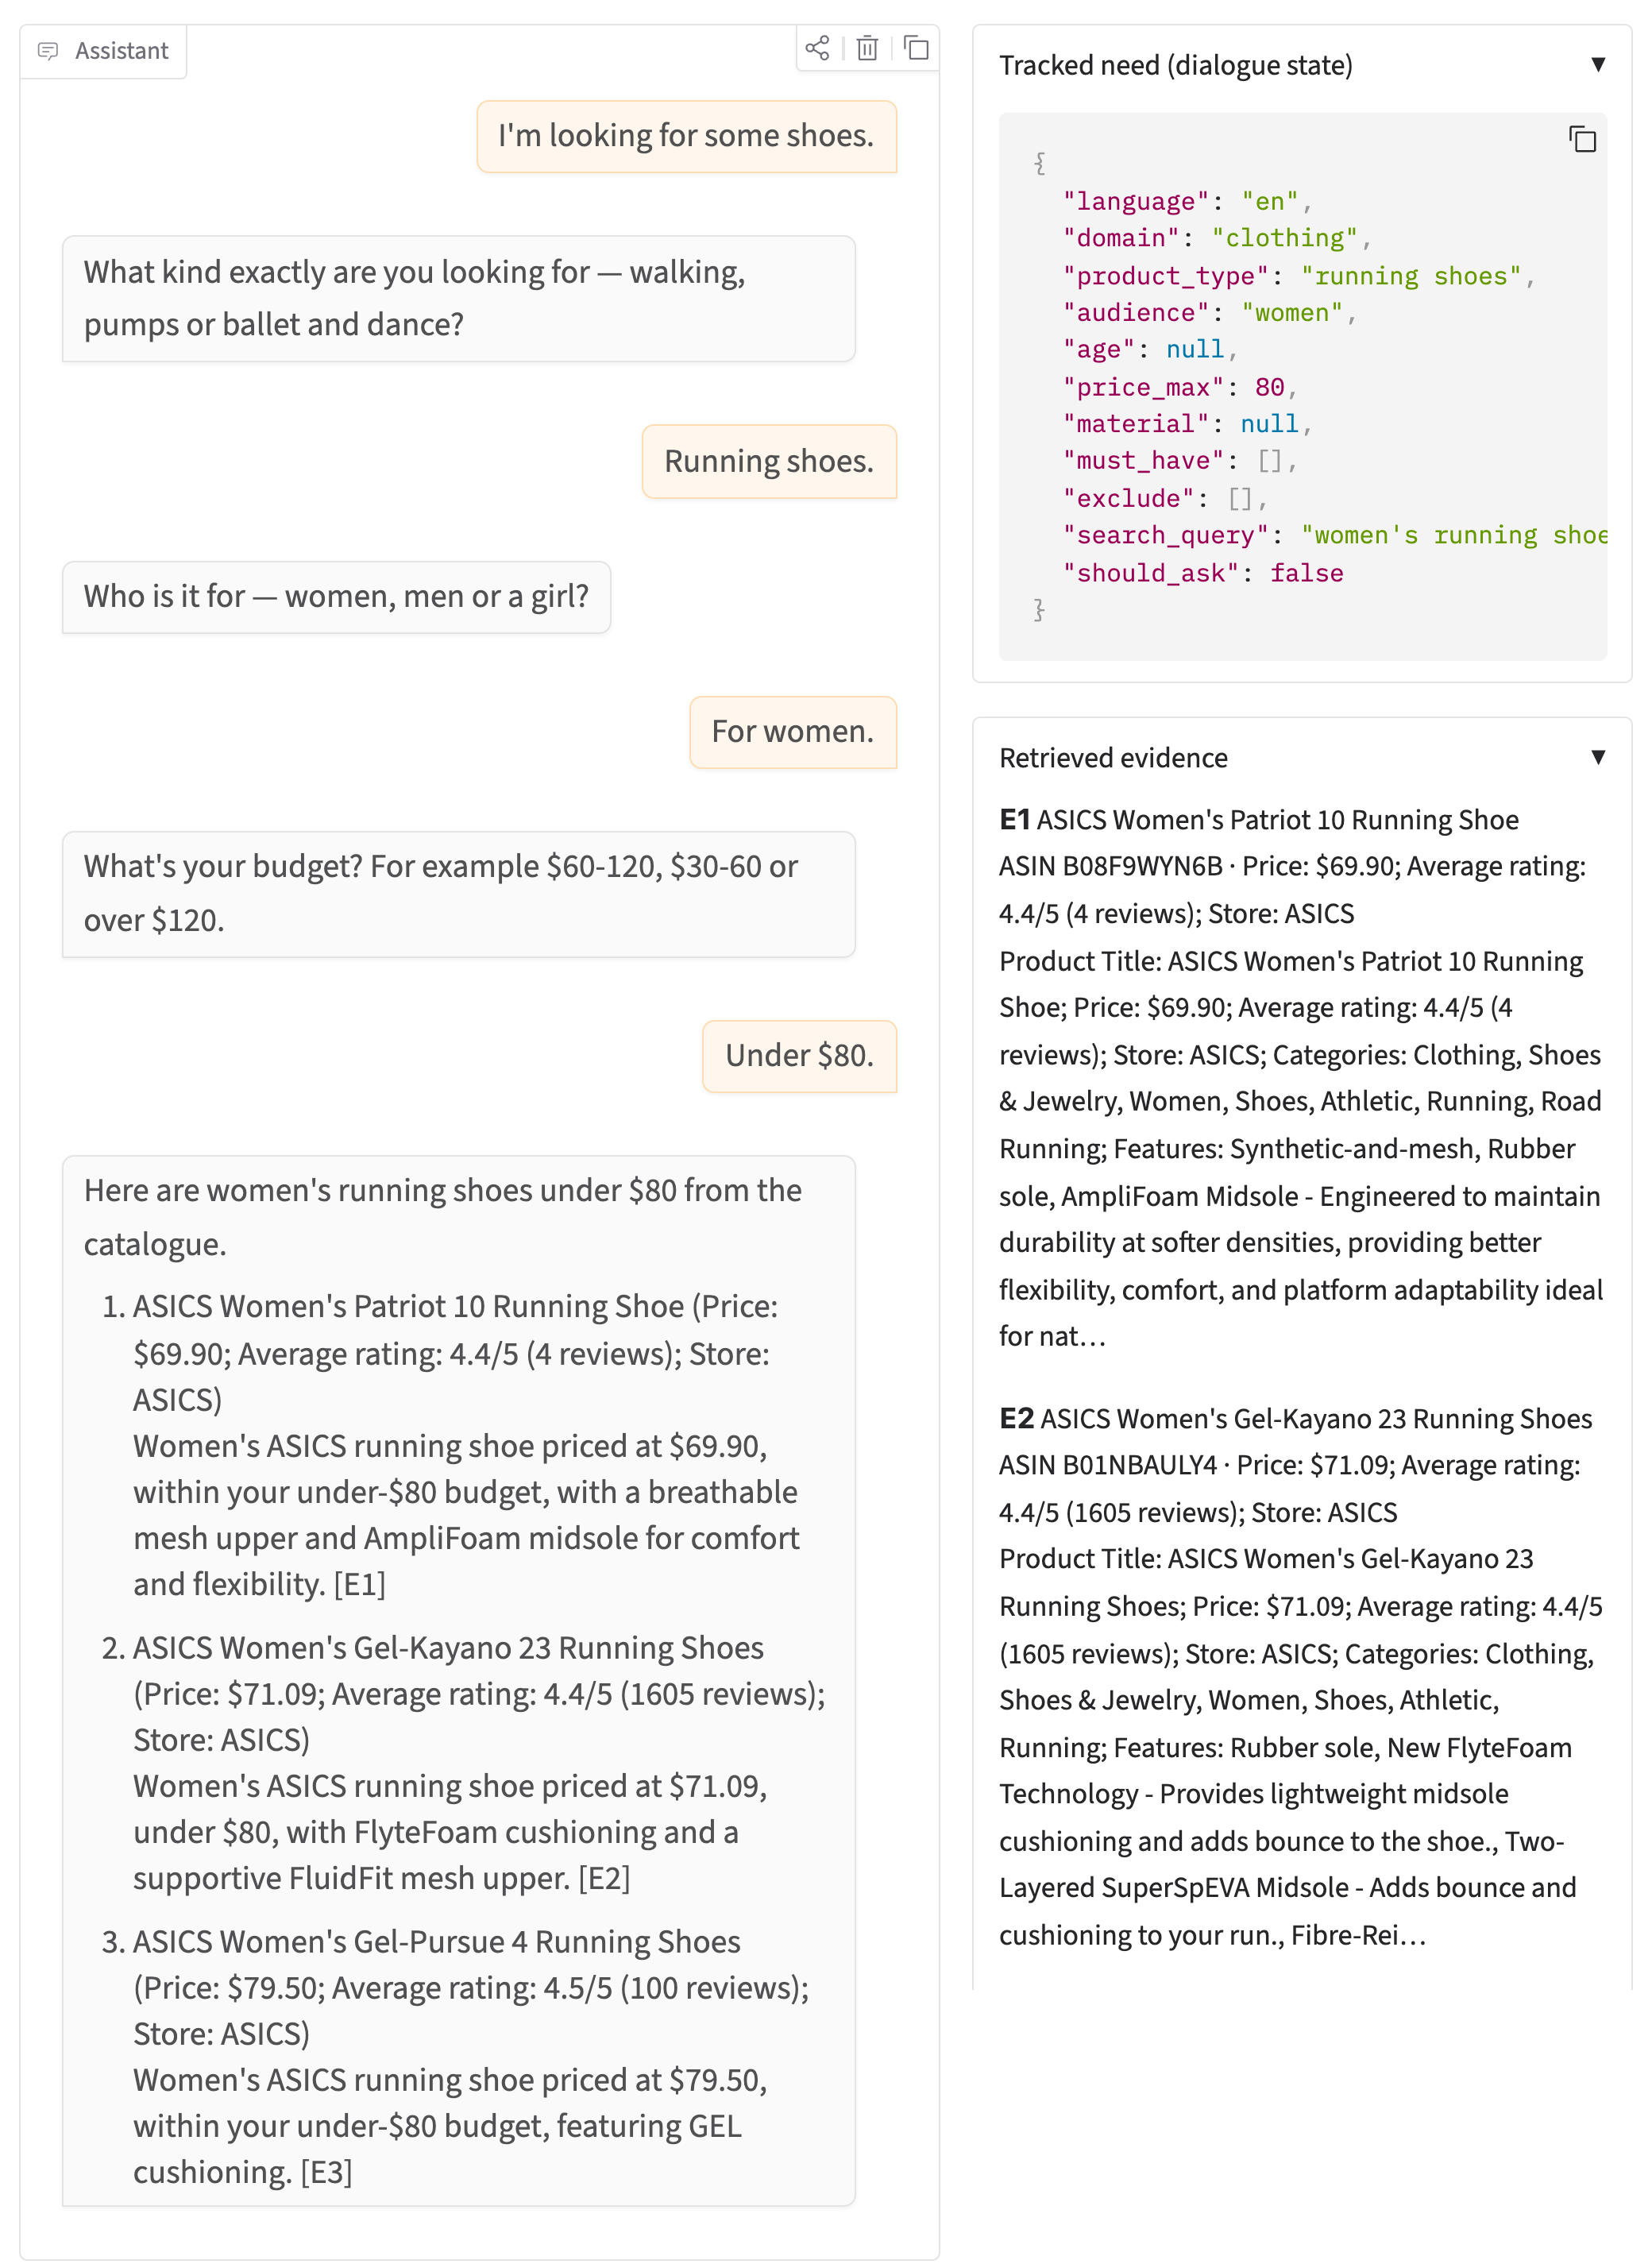
\includegraphics[width=0.74\textwidth]{figures/fig_ui.png}
\caption{The Gradio interface. Left: for ``I'm looking for some shoes'' the agent asks for the type, the wearer and the budget, then recommends three women's running shoes under \$80, each with price, rating, a reason and its evidence ID. Right: the tracked need (dialogue state) and the cited evidence passages.}
\label{fig:ui}
\end{figure*}

% =====================================================================
\section{Retrieval and Ranking Innovations (Q3)}
\textbf{Protocol.} Queries are the complete needs of the 169 unique evaluation scenarios (Section~\ref{sec:data}). We use two kinds of relevance: \emph{programmatic} qrels (every product satisfying all hard constraints of the need; complete, so recall is defined) and \emph{human} qrels on the 1,014 pooled candidates. Because only pooled products are judged, human P@5 is computed on the condensed list of judged products~\cite{sakai2007}. Programmatic labels agree with the human gold on 79.9\,\% of pairs ($\kappa{=}0.60$): precise (0.93) but strict, so their absolute values are conservative; both rank the configurations alike (Table~\ref{tab:retrieval}, Fig.~\ref{fig:retrieval}).

\begin{table*}[t]
\centering\small
\caption{Retrieval results on 169 queries. P@5, R@10, MRR@10 and nDCG@10 use programmatic qrels; the last two metric columns use human qrels. Chunk-level index unless stated.}
\label{tab:retrieval}
\begin{tabularx}{\textwidth}{@{}X rrrr rr r@{}}
\toprule
Configuration & P@5 & R@10 & MRR@10 & nDCG@10 & \makecell[r]{Human P@5\\(judged)} & \makecell[r]{Human\\nDCG@10} & \makecell[r]{Latency\\(ms)}\\
\midrule
BM25 & 0.369 & 0.180 & 0.521 & 0.381 & 0.618 & 0.426 & 0.3\\
Dense (bge-m3) & 0.420 & 0.187 & 0.612 & 0.421 & 0.624 & 0.533 & 22\\
RRF (equal weights) & 0.440 & 0.210 & 0.608 & 0.438 & 0.605 & 0.575 & 20\\
Weighted RRF (BM25 weight 0.5) & 0.451 & 0.213 & 0.619 & 0.449 & 0.635 & 0.558 & 20\\
RRF + cross-encoder re-ranking & 0.499 & 0.233 & 0.686 & 0.494 & 0.676 & 0.641 & 688\\
RRF + metadata filters & 0.656 & 0.332 & 0.770 & 0.660 & 0.862 & 0.634 & 22\\
RRF + re-ranking + filters & \textbf{0.698} & \textbf{0.356} & \textbf{0.826} & \textbf{0.705} & \textbf{0.895} & \textbf{0.792} & 787\\
\midrule
Product-level index: RRF + re-ranking + filters & \textbf{0.715} & \textbf{0.363} & \textbf{0.826} & \textbf{0.718} & \textbf{0.901} & 0.752 & 842\\
\midrule
Chinese query, dense & 0.151 & 0.064 & 0.299 & 0.154 & 0.360 & 0.221 & 21\\
Chinese query, RRF & 0.075 & 0.040 & 0.152 & 0.078 & 0.335 & 0.130 & 20\\
Chinese query, LLM-translated → RRF + re-ranking & 0.496 & 0.233 & 0.647 & 0.484 & 0.676 & 0.508 & 780\\
\bottomrule
\end{tabularx}
\end{table*}

\textbf{(1) Hybrid fusion.} BM25 matches exact attribute terms (``925 sterling silver''), dense retrieval matches paraphrases (``for my toddler'' $\approx$ ``ages 2+''). RRF beats both single retrievers on programmatic P@5 (0.440 vs.\ 0.369/0.420) and on human nDCG (0.575 vs.\ 0.426/0.533), but not on judged P@5; we therefore treat fusion mainly as a stronger candidate generator for the next two stages. Down-weighting BM25 helps slightly, down-weighting dense hurts.

\textbf{(2) Re-ranking.} The multilingual cross-encoder \code{bge-reranker-v2-m3} re-scores the top-20 fused products (+0.06 P@5, +0.08 MRR, +0.07 judged P@5) at 0.67\,s per query. For ``a wristwatch for women under \$220'' RRF returns a men's watch first (0/3 relevant in the top 3); after re-ranking all three are women's watches within budget.

\textbf{(3) Metadata and timeline search.} Embeddings do not encode ``under \$15'': for ``a coffee mug under \$15'' the RRF top 3 cost \$16.93–\$22.99. Applying budget, audience, age and material as filters on the top-200 candidates is the largest single gain (P@5 0.440 → 0.656; judged 0.605 → 0.862) at no latency cost. For time, adding ``released after 2021'' to the query text yields only 21.4\,\% compliant results, whereas a \code{date\_first\_available} filter yields 100\,\% and raises the share satisfying both date and need from 0.113 to 0.288.

\textbf{(4) Multilingual search.} bge-m3 embeds Chinese queries in the same space as English products, but direct Chinese retrieval is weak (P@5 0.151) and fusion makes it worse (0.075) because BM25 can only match digits: for \zh{“适合5岁孩子的积木，预算65美元以内”} BM25 matches ``65'' in ``1.65-inch'' die-cast cars. Translating the request to English with one LLM call recovers English quality (0.496 vs.\ 0.499), so the agent retrieves in English and answers in the user's language.

\textbf{(5) Chunking and indexing.} On need-style queries the product-level index is slightly better than field-level chunks (P@5 0.715 vs.\ 0.698), because type, audience and budget appear in every title and category path; chunks remain useful as citable evidence. Removing the BGE instruction prefix from documents (wrongly applied to both sides in our first version) was required for a valid index.

\begin{figure}[!htb]
\centering
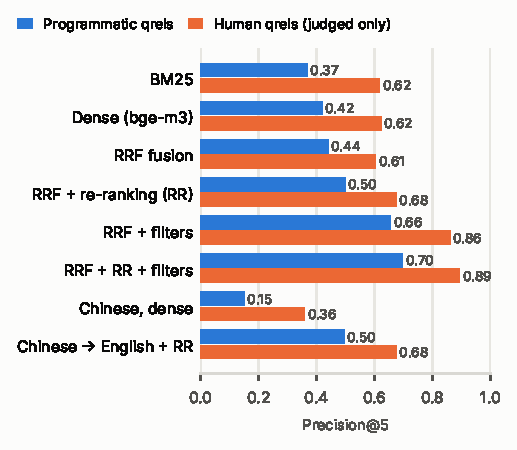
\includegraphics[width=\columnwidth]{figures/fig_retrieval.pdf}
\caption{Precision@5 of the main configurations under programmatic and human relevance judgments.}
\label{fig:retrieval}
\end{figure}

% =====================================================================
\section{Downstream Task and Generation (Q4)}
\subsection{Approach}
We use a retrieval-augmented LLM rather than a trained recommender: LLMs are strong zero-shot conversational recommenders when given item knowledge~\cite{he2023}, and our catalogue has no interaction data. Clarification follows the \emph{when to ask / what to ask} formulation of ClariQ~\cite{aliannejadi2020} and recent LLM work on proactive clarification~\cite{deng2023,zhang2025}. The generator returns JSON (answer, product IDs, evidence IDs); IDs not in the evidence are removed.

\textbf{Pre-processing.} Besides corpus cleaning (Q1), prices and ratings are injected after the title of each evidence passage so that truncating a long description never removes them, and colloquial or Chinese constraints (\zh{“50刀以内”} = under \$50) are normalised by the state tracker. Microtext normalisation is unnecessary for product metadata and short user messages.

\subsection{Evaluation dataset}\label{sec:data}
Each scenario has a hidden complete need (product type; audience, child age or material; budget) anchored on a real product and solvable by at least three catalogue products, and an opening message at one of three specificity levels, in English or Chinese. We label (i)~\emph{decision} records: for a dialogue snapshot, should the agent ask or recommend, and which attribute to ask about; and (ii)~\emph{relevance} records: does a pooled candidate (6 per scenario, from 7 retrieval configurations) satisfy the need. Of 180 generated scenarios, duplicates of an earlier need or dialogue are removed, leaving 169 scenarios, 299 decision and 1,014 relevance records (\textbf{1,313 unique records}; 68\,\%/32\,\% ask/recommend, 54\,\% relevant). Three group members labelled all records independently following written guidelines; the gold label is the majority vote. After one round of guideline clarification, in which one annotator re-checked the items labelled ``wrong product type'' (relevance agreement 79.9\,\% → 94.9\,\%; gold labels unchanged), agreement is high (Table~\ref{tab:iaa}).

\begin{table}[!htb]
\centering\small
\caption{Inter-annotator agreement (mean pairwise).}
\label{tab:iaa}
\begin{tabularx}{\columnwidth}{@{}X rrr@{}}
\toprule
Label & Records & Agreement & Fleiss' $\kappa$\\
\midrule
Ask or recommend & 299 & 98.7\,\% & 0.969\\
Attribute to ask about & 204 & 86.6\,\% & 0.812\\
Product satisfies the need & 1,014 & 94.9\,\% & 0.897\\
\textbf{All binary records} & \textbf{1,313} & \textbf{95.8\,\%} & \textbf{0.913}\\
\bottomrule
\end{tabularx}
\end{table}

\subsection{Task metrics}
\textbf{Clarification decision} (positive class = ask). The annotators followed the guideline ``ask if a required attribute is missing'', so the rule-based decision matches the gold on all snapshots; the learned criteria are compared in Table~\ref{tab:decision}. The entropy criterion never misses a needed question but over-asks in 50 of 95 recommend snapshots; LLM judgement misses 29\,\% of needed questions, and thinking mode recovers part of them. The attribute chosen to ask about matches the annotators only 52–58\,\% of the time, because the agent asks about the attribute that best splits the candidates rather than following the fixed priority type → audience/age → budget.

\begin{table}[!htb]
\centering\small
\caption{Ask/recommend decision against human gold (299 snapshots). The rule matches by construction, since the guidelines encode it.}
\label{tab:decision}
\begin{tabularx}{\columnwidth}{@{}X rrrr@{}}
\toprule
Criterion & P & R & F1 & \makecell[r]{Attribute\\acc.}\\
\midrule
Rule (required slot missing) & 1.000 & 1.000 & 1.000 & 0.583\\
LLM judgement & 0.973 & 0.711 & 0.822 & 0.517\\
LLM judgement + thinking & 0.972 & 0.838 & 0.900 & 0.538\\
Candidate entropy (ours) & 0.803 & 1.000 & 0.891 & 0.525\\
\bottomrule
\end{tabularx}
\end{table}

\textbf{Recommendation quality.} A rule-based user simulator (Section~\ref{sec:q5}) plays each scenario for at most five turns. The full agent succeeds (at least one of the top-3 products satisfies every hard constraint) in 87.6\,\% of dialogues and 85.2\,\% at the first recommendation, after 3.35 turns on average. Against the human labels, 93.7\,\% of its recommended products that fall in the judged pool are relevant (B0: 86.5\,\%); 37.2\,\% of recommended products violate at least one programmatically checked constraint, mostly unstated audience or age.

\subsection{Answer-level RAG metrics}
Following RAGAS~\cite{es2024}, an LLM judge scores the final answer of each dialogue. The full agent reaches \textbf{faithfulness 0.998}, answer relevance 0.604 and context precision 0.968 (single-turn baseline B0: 0.993, 0.548, 0.674); 95.2\,\% of numeric claims are verified against metadata, and all cited IDs are valid after validation. To check the judge, we applied its context-relevance prompt to the 1,014 human-labelled pairs: it agrees with the human gold on 92.7\,\% ($\kappa{=}0.853$), close to inter-annotator agreement.

\subsection{Performance}
Retrieval takes $\sim$20\,ms without and 0.7\,s with re-ranking; the per-turn latency of the full agent is 3.9\,s (p50) and 7.9\,s (p95), dominated by 2–3 LLM calls. A dialogue uses 7.0 LLM calls and $\sim$8.7k tokens, i.e.\ \$1.34 per 1,000 dialogues at DeepSeek off-peak prices with the 40\,\% context-cache hit rate observed on our bill (all experiments together cost \$4.61). With six parallel workers on one laptop the throughput is 0.39 dialogues/s, limited by API latency. For millions of products, FAISS IVF/HNSW or a vector database would replace exact search, the re-ranker would run batched on a GPU, and independent LLM calls of a turn could run in parallel.

% =====================================================================
\section{Downstream Innovations and Ablation (Q5)}\label{sec:q5}
\textbf{I1 — Clarification and information-gain question selection.} The agent asks when the unfilled attributes still split the top-30 candidates; it asks about the attribute with the highest value entropy and offers its most frequent values as options, a greedy retrieval-grounded form of information-gain question selection~\cite{hu2024,zou2020}. Without clarification the agent recommends blindly: for ``I need some clothes'', B1 lists a \$85 work set and 7 of its 9 listed products violate the hidden need, whereas the full agent asks for type, budget and wearer and recommends women's polo shirts under \$25 with no violation.

\textbf{I2 — Query rewriting and constraint-to-filter mapping.} Later turns (``cheaper, under 50 dollars'') are not searchable on their own; the dialogue is rewritten into a standalone query~\cite{mao2023} and hard constraints become metadata filters, relaxed step by step if no product survives. For ``a bracelet for women under \$40'', rewriting alone recommends a bracelet for teenage girls; with filters all three recommendations are women's bracelets $\leq$ \$40.

\textbf{I3 — Evidence check and claim-level self-check.} Before recommending, the agent checks that candidates satisfy the hard constraints and asks the LLM to confirm the match, relaxing and retrying if needed (in the spirit of CRAG~\cite{yan2024}); if nothing fits it says so (``I couldn't find a product that matches all of your requirements. Would you like to relax the budget?''). After generation, each claim is verified against its evidence and prices against metadata~\cite{dhuliawala2024}; e.g.\ the unsupported reason \zh{“适合聚会、通勤等多种场合”} is removed. Inspecting these examples also revealed a bug, the self-check rewriting the user's budget (``within your \$75 budget'' → ``\$21.80''), which we fixed.

\textbf{Simulator and protocol.} The user simulator knows only the hidden attribute values, never the target product, to avoid leaking the answer~\cite{zhu2024}; it answers only what is asked. Each configuration is run once on the 169 scenarios.

\begin{table*}[t]
\centering\small
\caption{Ablation on 169 simulated dialogues. Success@3: a top-3 product satisfies all hard constraints within five turns. Violations: share of recommended products violating a constraint. Decision F1 against human gold (Table~\ref{tab:decision}). Cost per 1,000 dialogues.}
\label{tab:ablation}
\begin{tabularx}{\textwidth}{@{}X rrrrrrrrr@{}}
\toprule
Configuration & Success@3 & \makecell[r]{First-rec.\\success} & Turns & Questions & Violations & \makecell[r]{Decision\\F1} & \makecell[r]{Faith-\\fulness} & \makecell[r]{LLM\\calls} & Cost\\
\midrule
B0 single-turn RAG (history concatenated) & 0.793 & 0.438 & 2.31 & 0 & 0.727 & 0 & 0.993 & 2.3 & \$0.73\\
B1 + query rewriting (I2) & 0.852 & 0.485 & 2.04 & 0 & 0.697 & 0 & 0.995 & 4.1 & \$0.92\\
B2 + LLM clarification & 0.858 & 0.763 & 2.72 & 1.22 & 0.558 & 0.822 & – & 5.4 & \$0.80\\
B3 + entropy clarification (I1) & 0.828 & 0.805 & 3.44 & 2.11 & 0.424 & 0.891 & – & 4.8 & \$0.77\\
B4 + metadata filters (I2) & 0.882 & \textbf{0.864} & 3.33 & 2.11 & 0.372 & 0.891 & 0.993 & 4.6 & \$0.74\\
\textbf{Full} = B4 + evidence check \& self-check (I3) & 0.876 & 0.852 & 3.35 & 2.11 & 0.372 & 0.891 & \textbf{0.998} & 7.0 & \$1.34\\
\midrule
Full − I1 (no clarification) & 0.586 & 0.485 & 1.39 & 0 & 0.580 & 0 & – & 5.2 & \$1.13\\
Full − I2 (no rewriting, no filters) & 0.852 & 0.834 & 3.38 & 2.11 & 0.369 & 0.891 & – & 7.1 & \$1.23\\
Full − I3 & \textbf{0.888} & \textbf{0.864} & 3.33 & 2.11 & 0.383 & 0.891 & 0.995 & 4.6 & \$0.74\\
\midrule
Full, rule-based decision & 0.882 & 0.799 & 3.05 & 1.71 & 0.427 & 1.000 & – & 7.0 & \$1.40\\
Full, random question choice & 0.876 & 0.834 & 3.40 & 2.12 & 0.381 & 0.891 & – & 7.2 & \$1.38\\
Full + DeepSeek thinking mode & \textbf{0.893} & \textbf{0.864} & 3.33 & 2.13 & \textbf{0.332} & – & – & 6.9 & \$1.77\\
\bottomrule
\end{tabularx}
\end{table*}

\begin{figure*}[t]
\centering
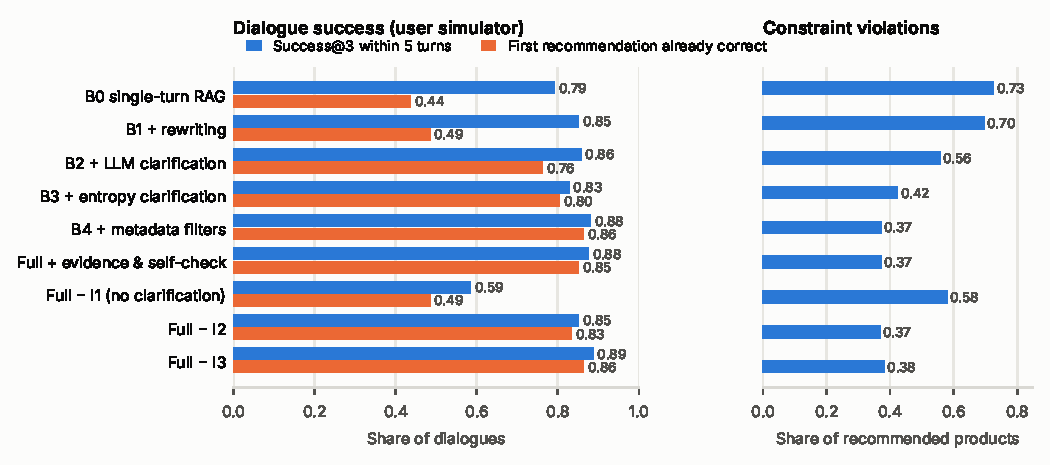
\includegraphics[width=\textwidth]{figures/fig_ablation.pdf}
\caption{Ablation of the downstream innovations: dialogue success (left) and constraint violations (right).}
\label{fig:ablation}
\end{figure*}

\textbf{Findings} (Table~\ref{tab:ablation}, Fig.~\ref{fig:ablation}).
\begin{itemize}
\item \emph{Clarification is the main driver}: removing it drops success from 0.876 to 0.586, and adding it to B1 raises first-recommendation success from 0.485 to 0.763.
\item \emph{Constraint filters} mainly reduce violations (B3 → B4: 0.424 → 0.372) and raise success (0.828 → 0.882).
\item \emph{Entropy decisions over-ask}: on fully specified openings the agent still asks in half of the cases (``a ring for women under \$25'' → ``statement, stacking or bands?''). The rule-based decision reaches similar success with fewer and more useful questions (96.5\,\% vs.\ 81.2\,\% useful), and entropy-based \emph{selection} is no better than choosing a random missing attribute (0.876 both) — with only 3–5 slots any missing required slot is informative.
\item \emph{Grounding checks (I3)} do not change simulator success (0.888 vs.\ 0.876 is within the noise of a single run) but give the highest faithfulness and turn invented matches into honest refusals, at 2.4 extra LLM calls (+\$0.6 per 1,000 dialogues).
\item \emph{Thinking mode} gives the fewest violations (0.332) at 33\,\% higher cost. Aspect-level explanations (an optional I4) did not help (success 0.870, fewer verified claims).
\end{itemize}

% =====================================================================
\section{Limitations}
The catalogue contains metadata but no reviews, so subjective aspects (comfort, fit) are supported only when stated in a listing. The same LLM family acts as agent, simulator and judge; we calibrate the judge against human labels. Human relevance labels cover only pooled products, so human retrieval metrics are computed on judged products. Each configuration was run once, so small differences (around $\pm$0.01) are not significant.

% =====================================================================
\footnotesize
\begin{thebibliography}{99}\setlength{\itemsep}{0pt}
\bibitem{aliannejadi2020} M.~Aliannejadi et al. ConvAI3: Generating clarifying questions for open-domain dialogue systems (ClariQ). arXiv:2009.11352, 2020.
\bibitem{cormack2009} G.~V.~Cormack, C.~L.~A.~Clarke, S.~Büttcher. Reciprocal rank fusion outperforms Condorcet and individual rank learning methods. SIGIR 2009.
\bibitem{deng2023} Y.~Deng et al. Prompting and evaluating large language models for proactive dialogues: clarification, target-guided, and non-collaboration. Findings of EMNLP 2023.
\bibitem{dhuliawala2024} S.~Dhuliawala et al. Chain-of-verification reduces hallucination in large language models. Findings of ACL 2024.
\bibitem{es2024} S.~Es et al. RAGAS: Automated evaluation of retrieval augmented generation. EACL 2024 (demo).
\bibitem{he2023} Z.~He et al. Large language models as zero-shot conversational recommenders. CIKM 2023.
\bibitem{hou2024} Y.~Hou et al. Bridging language and items for retrieval and recommendation. arXiv:2403.03952, 2024.
\bibitem{hu2024} Z.~Hu et al. Uncertainty of thoughts: uncertainty-aware planning enhances information seeking in large language models. NeurIPS 2024.
\bibitem{mao2023} K.~Mao et al. Large language models know your contextual search intent: a prompting framework for conversational search. Findings of EMNLP 2023.
\bibitem{sakai2007} T.~Sakai. Alternatives to Bpref. SIGIR 2007.
\bibitem{yan2024} S.-Q.~Yan et al. Corrective retrieval augmented generation. arXiv:2401.15884, 2024.
\bibitem{zhang2025} M.~J.~Q.~Zhang, E.~Choi. Clarify when necessary: resolving ambiguity through interaction with LMs. Findings of NAACL 2025.
\bibitem{zhu2024} L.~Zhu et al. How reliable is your simulator? An analysis on the limitations of current LLM-based user simulators for conversational recommendation. WWW 2024 Companion.
\bibitem{zou2020} J.~Zou, Y.~Chen, E.~Kanoulas. Towards question-based recommender systems. SIGIR 2020.
\end{thebibliography}

\end{document}
